\section{Durchführung}
\label{sec:Durchführung}
Der Pumpstand wird wie in Abbildung \ref{fig:Aufbau} aufgebaut. Dabei ist es wichtig möglichst genau 
zu arbeiten, damit keine Lecks durch falsch angebrachte Gummis und Flansches entstehen. Danach wird 
der Pumpstand mit der Drehschieberpumpe evakuiert. Stellt sich nach ca. 10 Minuten ein Druck 
zwischen 3 und \SI{5}{\hecto\pascal} ein, dann kann die Turbopumpe hinzugeschaltet werden. 
Erst jetzt wird das Glühkathoden-Vakuummeter eingeschaltet, da es sonst durchbrennen könnte.
Dann wird der Rezipient ca. 15 Minuten mit einem Heißluftföhn erwärmt. Das 
führt dazu, dass Wasserablagerungen im Rezipienten ausdampfen und die Desorptionsrate 
abnimmt. Bei starker Wasseransammlung, kann ein Gasanfall beobachtet werden, sofern die 
Messgeräte eingeschaltet sind. Wird nun ein Enddruck zwischen \SI{2e-3}{} und \SI{8e-3}{\pascal} 
erreicht gilt der Aufbau als dicht und es kann mit der Messung angefangen werden.
\newline
\newline
Da der Enddruck des Aufbaus erreicht ist und die Turbopumpe schon arbeitet, bietet es sich an 
mit der Messung zur Turbopumpe anzufangen. Zur Messung der Evakuierungspumpe wird über das 
Nadel- und Kugelventiel bis zu einem Druck von \SI{0.5}{\pascal} belüftet. Dann werden beide 
Ventile, möglichst zeitgleich, geschlossen und die Messung beginnt. Nun wird der Druckabfall in 
Abhängigkeit von der Zeit gemessen. Die Messung wird fünfmal wiederholt. Die Messzeit beträgt 
jeweils \SI{120}{\second}. Die Messung erfolgt über das Glühkathoden-Vakuummeter.
\newline 
\newline 
Für die Leckratenmessung wird im Rezipienten ein Gleichgewichtsdruck zwischen \SI{5e-3}{} 
und \SI{20e-3}{\pascal} eingestellt. Danach wird sowohl die Turbopumpe als auch die 
Drehschieberpumpe abgeschiebert. Die Messung wird jeweils dreimal durchgeführt. Zudem werden 
vier Leckraten gemessen, folglich vier Gleichgewichtsdrücke eingestellt. Auch hier erfolgt die 
Messung über das Glühkathoden-Vakuummeter. 
\newline
\newline
Um die Messung für die Drehschieberpumpe beginnen zu können muss zuerst das Glühkathoden-Vakuummeter 
abgeschaltet werden und die Turbopumpe abgeschiebert werden. Dann wird die Messung analog 
zur Turbopumpe durchgeführt. Natürlich werden die Druckbereiche der Evakuierungskurvenmessung 
und der Leckratenmessung angepasst. Genauer beträgt der Druck nach Belüftung für die 
Messung der Evakuierungskurve jetzt ca. \SI{1000}{\hecto\pascal}, also Normaldruck. Der 
Druckbereich der Gleichgewichtsdrücke liegt für die Leckratenmessung bei \SI{0.1}{} und 
\SI{1}{\hecto\pascal}. Für die Messung der Evakuierungskurve wird das analoge und für 
die Leckratenmessung das digitale Pirani-Vakuummeter verwendet. 
\newline
\newline
Nach Durchführung der Messungen wird der Aufbau abgebaut und der Rezipient sowie die Pumpen 
werden abgestellt und mit Flanschen verschlossen, um die Verunreihnigung durch Ad- und Absorption 
gering zuhalten. Danach werden alle im Aufbau verwendeten Teile vermessen, um später das effektiv 
evakuierte Volumen berechnen zu können.
\begin{SCfigure}
  \caption[justification=raggedleft]{Foto des Versuchsaufbaus mit nummerierten Komponenten; \\
1. Rezipient\\
2. Dosierventiel, auch Nadelventil\\
3,5. Kugelventiel \\
4. Glühkathodenvakuummeter\\
6. Turbomolekularpumpe\\
7. Pirani-Digitalvakuummeter\\
8. Pirani-Analogvakuummeter\\
9,11. Schlauch\\
10. Drehschieberpumpe\\
12. Kreuzstück, \\
an dem ein Rohr mit 7. und 8., \\
die Schläuche 9. und 11.\\
 und ein Kugelventil \\
 zur Turbopumpe befestigt ist.\\
13. Anzeigen von 4. und 8. \\
14. Steuergerät der Turbopumpe \\
}
  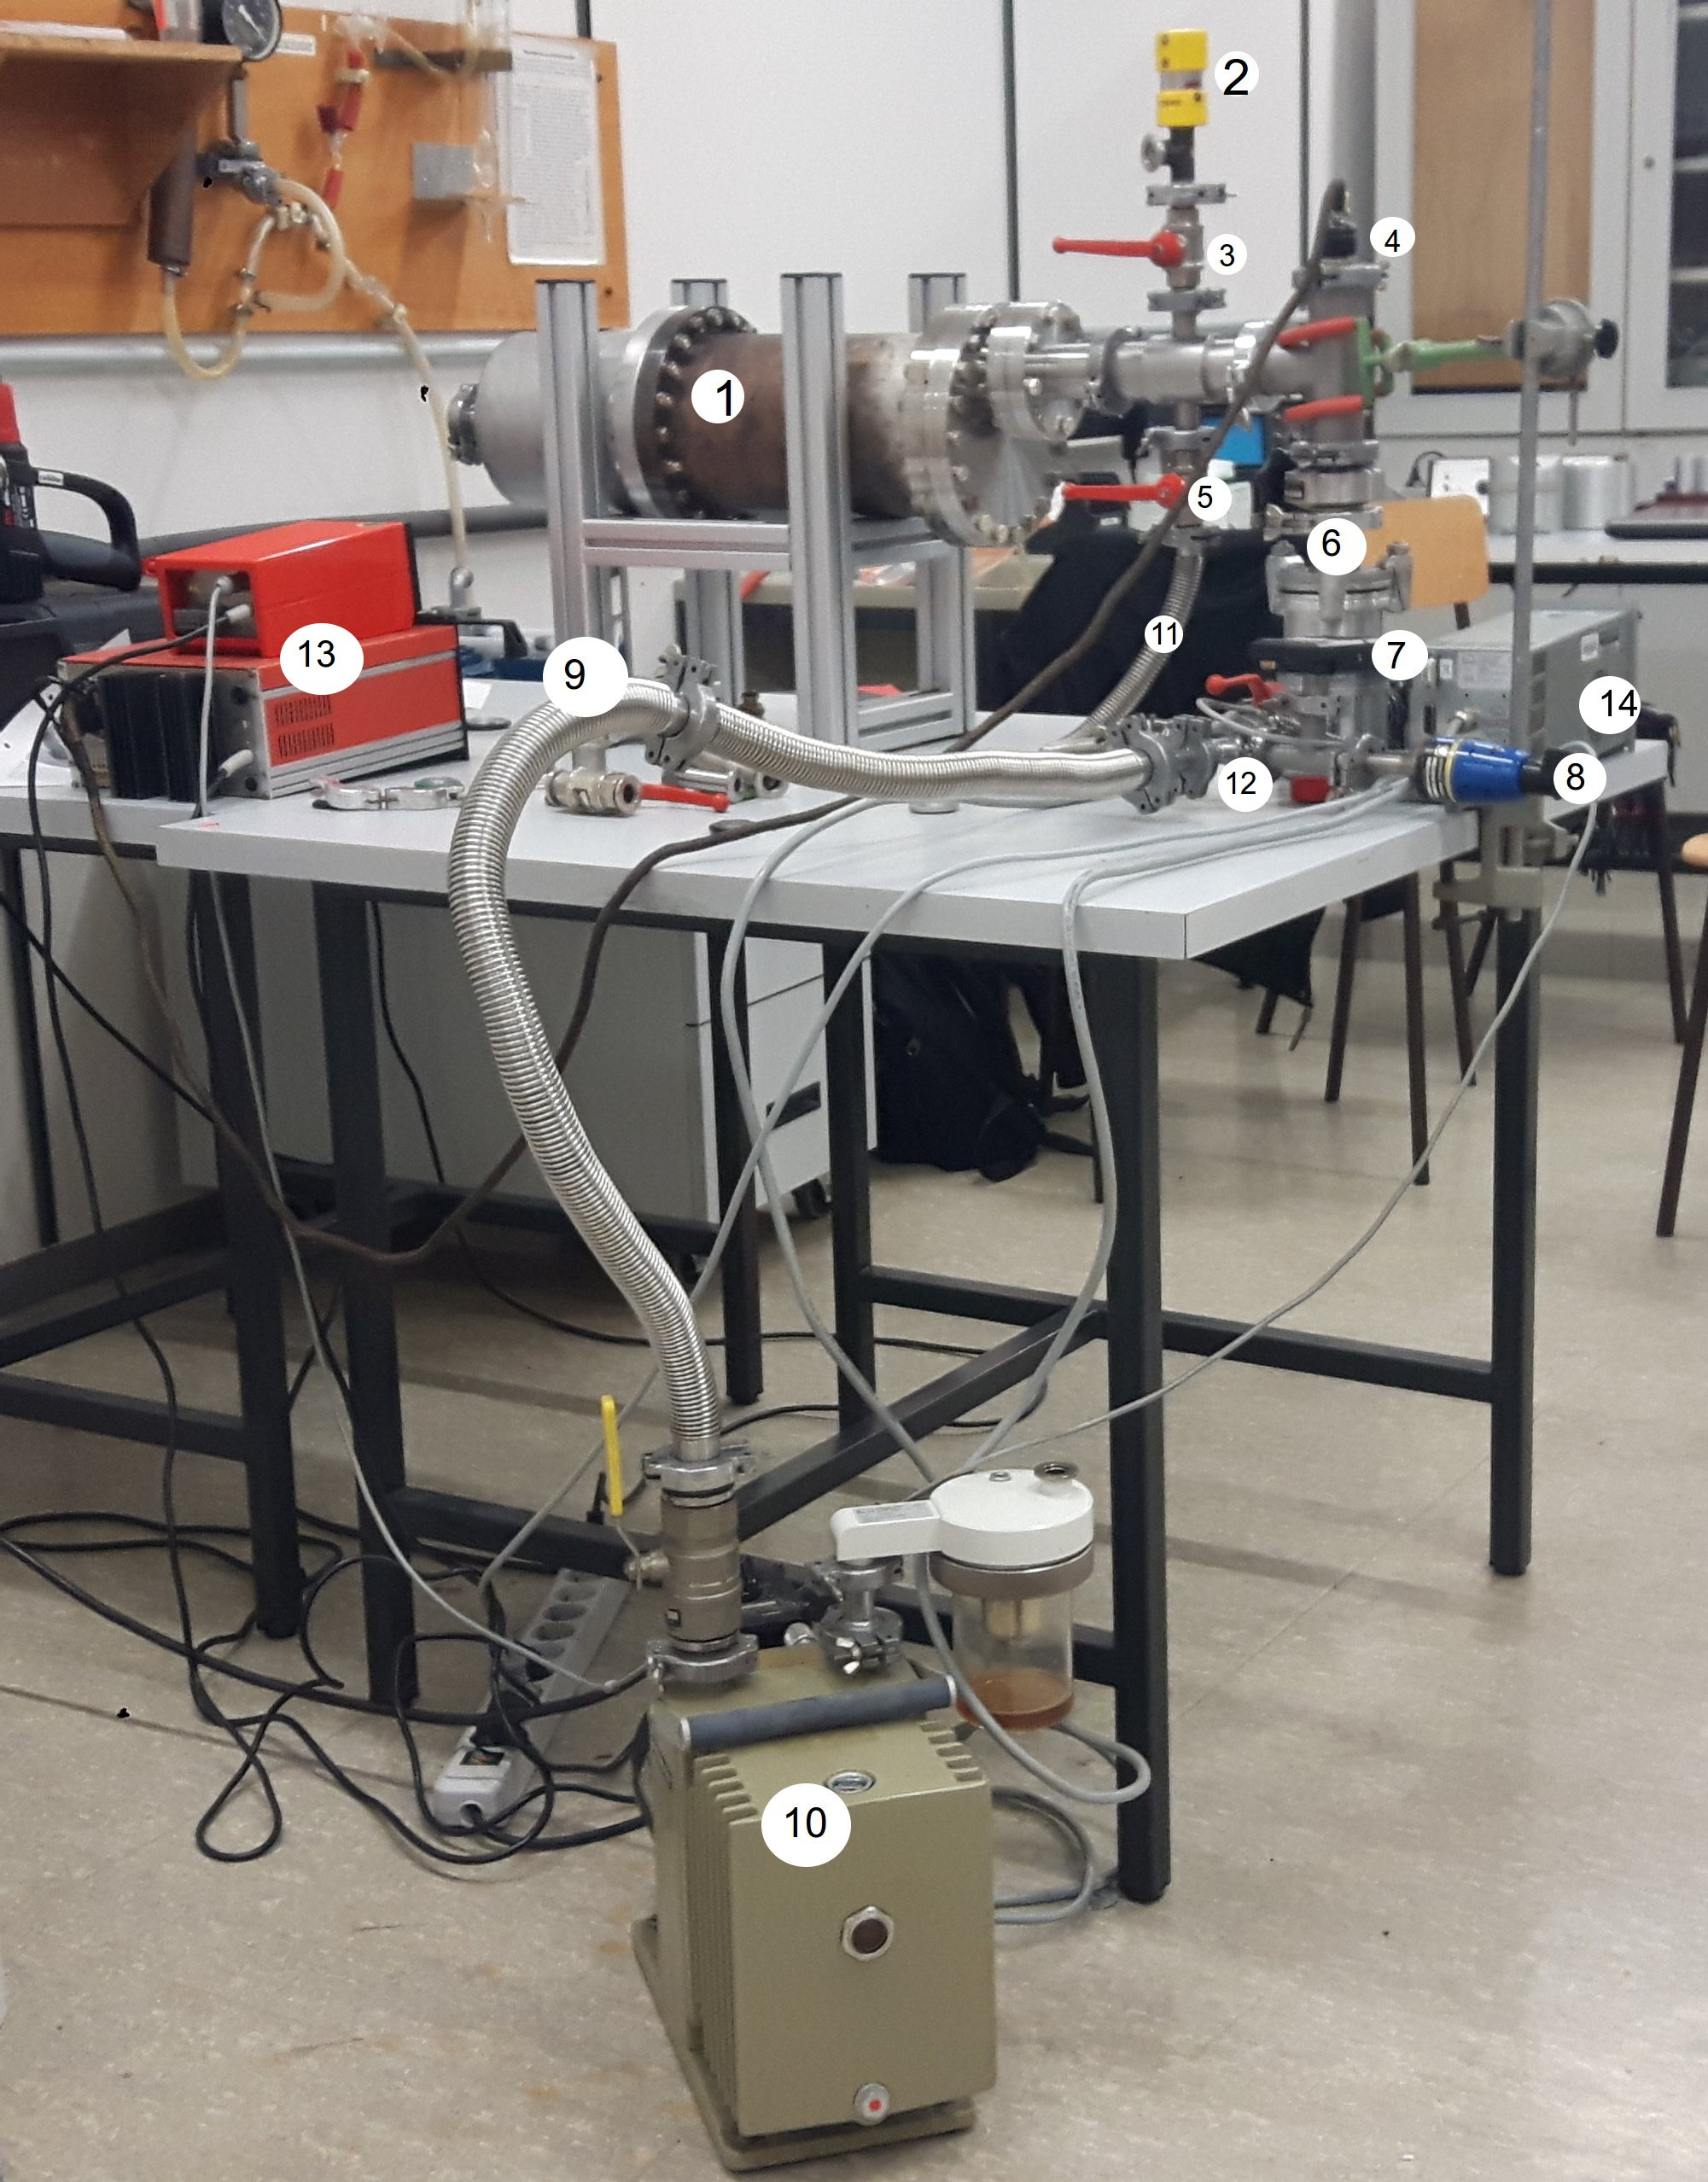
\includegraphics[height  = 10cm]{pics/V3B2.jpg}
  \label{fig:Aufbau}
\end{SCfigure}


